\documentclass{article}
\usepackage[utf8]{inputenc}
\usepackage{graphicx}
\usepackage{booktabs}
\usepackage{float}
\graphicspath{ {./metrics/fold_0/} }
\graphicspath{ {./metrics/fold_1/} }
\graphicspath{ {./metrics/fold_2/} }
\title{Results: bert-base-uncased-baseline-lr-[0.00005|0.00001|0.000001]}
\author{Nadia Sheikh}
\date{2022-07-25}
\begin{document}
\maketitle
\section{Configurations}
\subsection{Run Configuration}
\begin{tabular}{ll}
\toprule
{} &                                                  0 \\
\midrule
experiment\_identifier &                          llm-baseline-[bert|sbert] \\
run\_identifier        &  bert-base-uncased-baseline-lr-[0.00005|0.00001... \\
config\_file\_path      &  /tmp/71317.1.all.q/ctre/cnc-task-3/script-deve... \\
\bottomrule
\end{tabular}

\subsection{Data Configuration}
\begin{tabular}{ll}
\toprule
{} &                                                  0 \\
\midrule
data\_utility\_cls        &                                      cnc\_utilities \\
dataset\_cls             &                                   CNCTask3aDataset \\
nos\_of\_folds            &                                                  3 \\
trn\_data\_path           &    /cnc-task-3/script-development/data/CSV-Output/ \\
tst\_data\_path           &  /home/nadia/Documents/CLaC-Lab/ctre/cnc-task-3... \\
base\_output\_folder\_path &             /cnc-task-3/script-development/output/ \\
config\_file\_path        &  /tmp/71317.1.all.q/ctre/cnc-task-3/script-deve... \\
\bottomrule
\end{tabular}

\subsection{Preprocessing Configuration}
\begin{tabular}{ll}
\toprule
{} &                                                  0 \\
\midrule
collate\_fn\_name   &                                       LLMCollateFn \\
llm\_name          &                                  bert-base-uncased \\
connl\_folder\_path &  /home/nadia/Documents/CLaC-Lab/ctre/cnc-task-3... \\
max\_nos\_tokens    &                                                 84 \\
token\_sep         &                                               True \\
config\_file\_path  &  /tmp/71317.1.all.q/ctre/cnc-task-3/script-deve... \\
\bottomrule
\end{tabular}

\section{Hyperparameters}
\subsection{hparam\_config\_id\_0}
\begin{tabular}{ll}
\toprule
{} &                   0 \\
\midrule
loss\_function                    &  cross-entropy-loss \\
learning\_rate                    &             0.00005 \\
batch\_size                       &                   1 \\
optimizer                        &                adam \\
llm                              &   bert-base-uncased \\
llm\_hidden\_dropout\_prob          &                 0.1 \\
llm\_attention\_probs\_dropout\_prob &                 0.1 \\
pooling                          &                 cls \\
classes                          &                   2 \\
max\_epochs                       &                   3 \\
\bottomrule
\end{tabular}

\subsection{hparam\_config\_id\_1}
\begin{tabular}{ll}
\toprule
{} &                   0 \\
\midrule
loss\_function                    &  cross-entropy-loss \\
learning\_rate                    &             0.00001 \\
batch\_size                       &                   1 \\
optimizer                        &                adam \\
llm                              &   bert-base-uncased \\
llm\_hidden\_dropout\_prob          &                 0.1 \\
llm\_attention\_probs\_dropout\_prob &                 0.1 \\
pooling                          &                 cls \\
classes                          &                   2 \\
max\_epochs                       &                   3 \\
\bottomrule
\end{tabular}

\subsection{hparam\_config\_id\_2}
\begin{tabular}{ll}
\toprule
{} &                   0 \\
\midrule
loss\_function                    &  cross-entropy-loss \\
learning\_rate                    &            0.000005 \\
batch\_size                       &                   1 \\
optimizer                        &                adam \\
llm                              &   bert-base-uncased \\
llm\_hidden\_dropout\_prob          &                 0.1 \\
llm\_attention\_probs\_dropout\_prob &                 0.1 \\
pooling                          &                 cls \\
classes                          &                   2 \\
max\_epochs                       &                   3 \\
\bottomrule
\end{tabular}

\section{fold\_0}
\subsection{train\_loss}
\begin{tabular}{lrrr}
\toprule
{} &   ep 0 &   ep 1 &   ep 2 \\
\midrule
hp\_0 &  0.796 &  0.718 &  0.745 \\
hp\_1 &  0.677 &  0.301 &  0.039 \\
hp\_2 &  0.687 &  0.410 &  0.094 \\
\bottomrule
\end{tabular}

\begin{figure}[H]
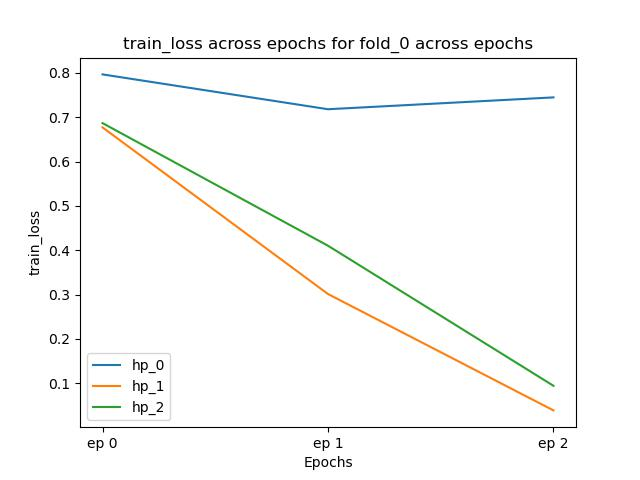
\includegraphics[scale = 0.75]{fold_0/train_loss}
\end{figure}
\subsection{test\_loss}
\begin{tabular}{lrrr}
\toprule
{} &   ep 0 &   ep 1 &   ep 2 \\
\midrule
hp\_0 &  0.692 &  1.491 &  0.693 \\
hp\_1 &  0.543 &  0.285 &  0.305 \\
hp\_2 &  0.591 &  0.420 &  0.404 \\
\bottomrule
\end{tabular}

\begin{figure}[H]
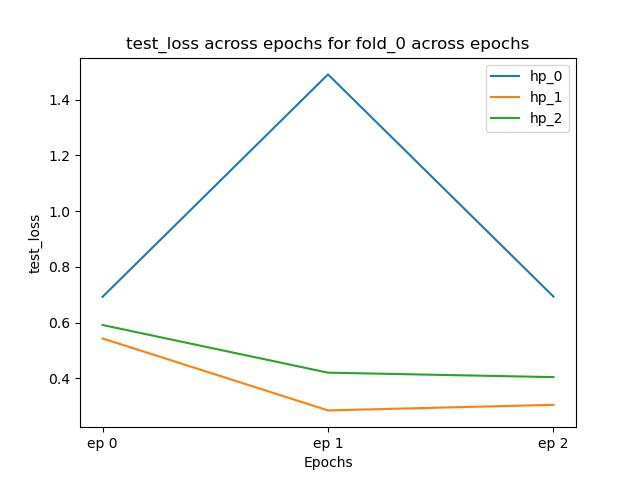
\includegraphics[scale = 0.75]{fold_0/test_loss}
\end{figure}
\subsection{accuracy\_score}
\begin{tabular}{lrrr}
\toprule
{} &   ep 0 &   ep 1 &   ep 2 \\
\midrule
hp\_0 &  0.521 &  0.521 &  0.521 \\
hp\_1 &  0.778 &  0.863 &  0.889 \\
hp\_2 &  0.692 &  0.795 &  0.812 \\
\bottomrule
\end{tabular}

\begin{figure}[H]
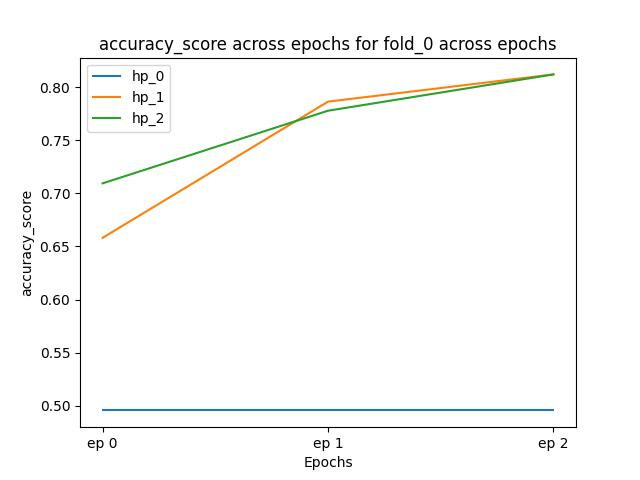
\includegraphics[scale = 0.75]{fold_0/accuracy_score}
\end{figure}
\subsection{f1\_score}
\begin{tabular}{lrrr}
\toprule
{} &   ep 0 &   ep 1 &   ep 2 \\
\midrule
hp\_0 &  0.000 &  0.000 &  0.000 \\
hp\_1 &  0.780 &  0.855 &  0.876 \\
hp\_2 &  0.591 &  0.778 &  0.788 \\
\bottomrule
\end{tabular}

\begin{figure}[H]
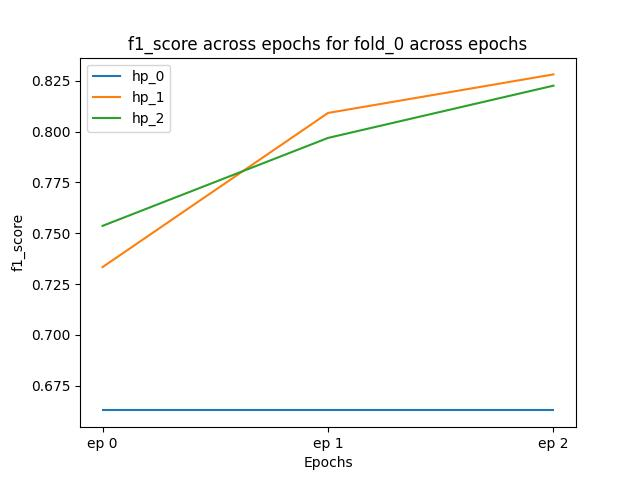
\includegraphics[scale = 0.75]{fold_0/f1_score}
\end{figure}
\subsection{precision\_score}
\begin{tabular}{lrrr}
\toprule
{} &   ep 0 &   ep 1 &   ep 2 \\
\midrule
hp\_0 &  0.000 &  0.000 &  0.000 \\
hp\_1 &  0.742 &  0.870 &  0.939 \\
hp\_2 &  0.812 &  0.808 &  0.854 \\
\bottomrule
\end{tabular}

\begin{figure}[H]
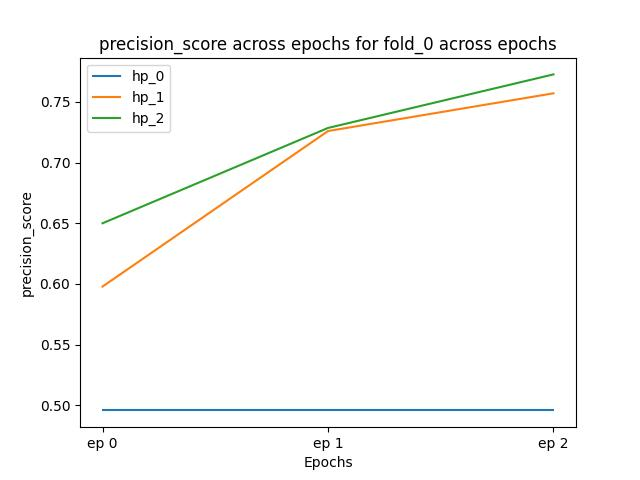
\includegraphics[scale = 0.75]{fold_0/precision_score}
\end{figure}
\subsection{matthews\_corrcoef}
\begin{tabular}{lrrr}
\toprule
{} &  ep 0 &   ep 1 &   ep 2 \\
\midrule
hp\_0 &  0.00 &  0.000 &  0.000 \\
hp\_1 &  0.56 &  0.726 &  0.782 \\
hp\_2 &  0.41 &  0.589 &  0.627 \\
\bottomrule
\end{tabular}

\begin{figure}[H]
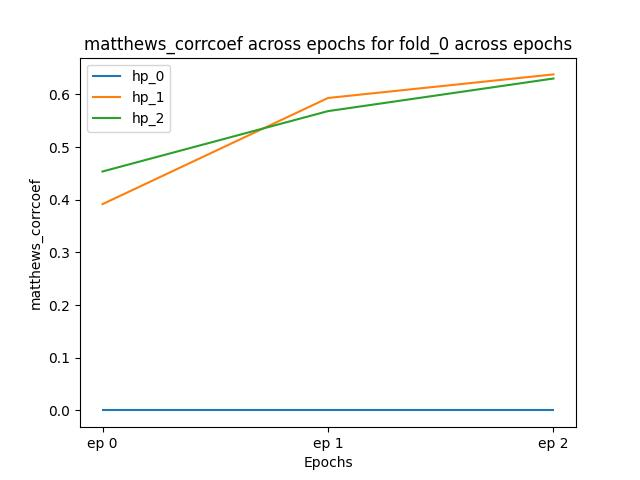
\includegraphics[scale = 0.75]{fold_0/matthews_corrcoef}
\end{figure}
\subsection{recall\_score}
\begin{tabular}{lrrr}
\toprule
{} &   ep 0 &   ep 1 &   ep 2 \\
\midrule
hp\_0 &  0.000 &  0.000 &  0.000 \\
hp\_1 &  0.821 &  0.839 &  0.821 \\
hp\_2 &  0.464 &  0.750 &  0.732 \\
\bottomrule
\end{tabular}

\begin{figure}[H]
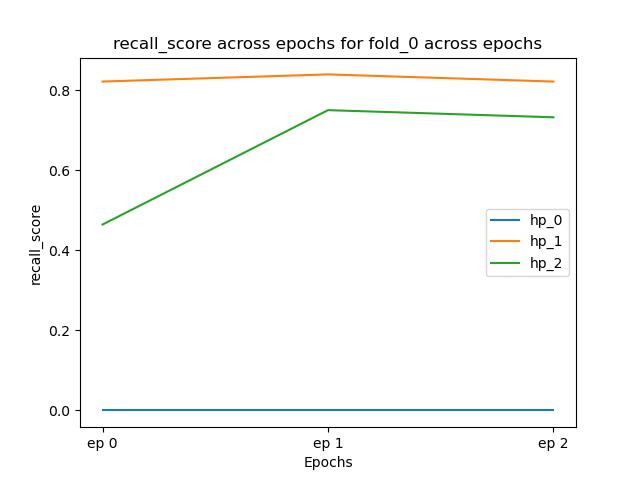
\includegraphics[scale = 0.75]{fold_0/recall_score}
\end{figure}
\section{fold\_1}
\subsection{train\_loss}
\begin{tabular}{lrrr}
\toprule
{} &   ep 0 &   ep 1 &   ep 2 \\
\midrule
hp\_0 &  0.746 &  0.669 &  0.403 \\
hp\_1 &  0.691 &  0.270 &  0.020 \\
hp\_2 &  0.666 &  0.389 &  0.077 \\
\bottomrule
\end{tabular}

\begin{figure}[H]
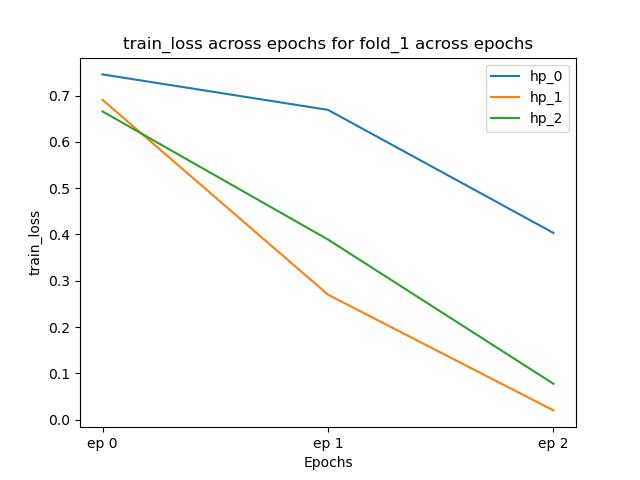
\includegraphics[scale = 0.75]{fold_1/train_loss}
\end{figure}
\subsection{test\_loss}
\begin{tabular}{lrrr}
\toprule
{} &   ep 0 &   ep 1 &   ep 2 \\
\midrule
hp\_0 &  0.712 &  0.564 &  0.460 \\
hp\_1 &  0.553 &  0.357 &  0.357 \\
hp\_2 &  0.586 &  0.384 &  0.390 \\
\bottomrule
\end{tabular}

\begin{figure}[H]
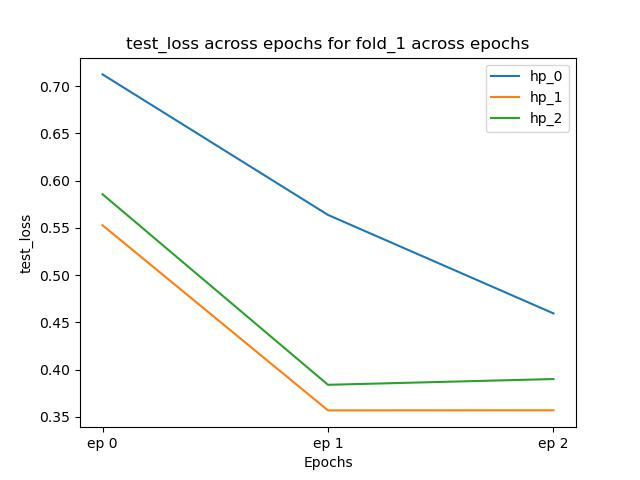
\includegraphics[scale = 0.75]{fold_1/test_loss}
\end{figure}
\subsection{accuracy\_score}
\begin{tabular}{lrrr}
\toprule
{} &   ep 0 &   ep 1 &   ep 2 \\
\midrule
hp\_0 &  0.466 &  0.681 &  0.793 \\
hp\_1 &  0.759 &  0.836 &  0.828 \\
hp\_2 &  0.741 &  0.819 &  0.819 \\
\bottomrule
\end{tabular}

\begin{figure}[H]
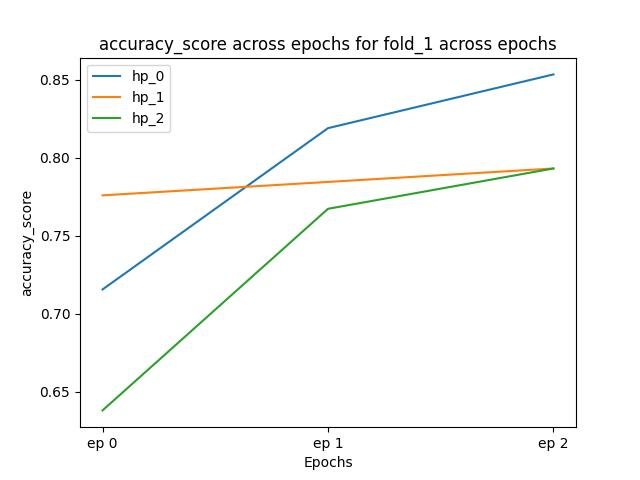
\includegraphics[scale = 0.75]{fold_1/accuracy_score}
\end{figure}
\subsection{f1\_score}
\begin{tabular}{lrrr}
\toprule
{} &   ep 0 &   ep 1 &   ep 2 \\
\midrule
hp\_0 &  0.000 &  0.761 &  0.815 \\
hp\_1 &  0.759 &  0.850 &  0.828 \\
hp\_2 &  0.706 &  0.821 &  0.817 \\
\bottomrule
\end{tabular}

\begin{figure}[H]
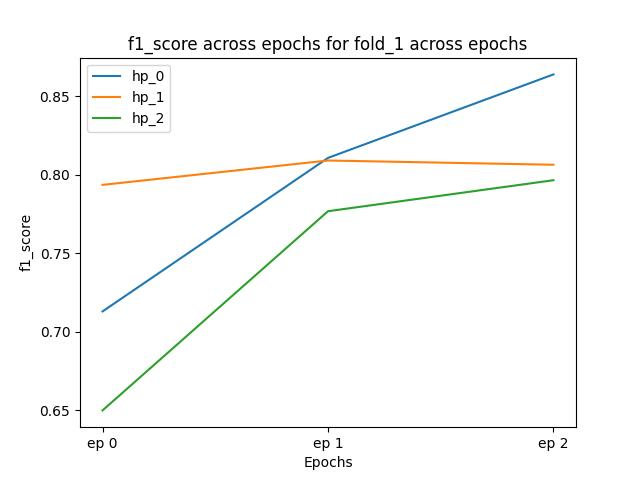
\includegraphics[scale = 0.75]{fold_1/f1_score}
\end{figure}
\subsection{precision\_score}
\begin{tabular}{lrrr}
\toprule
{} &   ep 0 &   ep 1 &   ep 2 \\
\midrule
hp\_0 &  0.000 &  0.634 &  0.779 \\
hp\_1 &  0.815 &  0.831 &  0.889 \\
hp\_2 &  0.900 &  0.873 &  0.887 \\
\bottomrule
\end{tabular}

\begin{figure}[H]
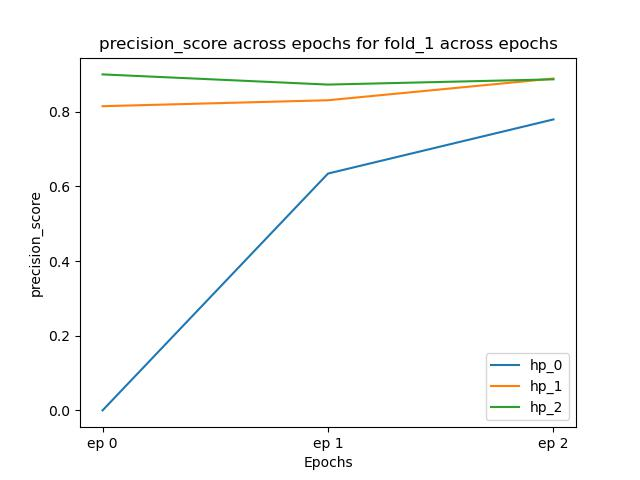
\includegraphics[scale = 0.75]{fold_1/precision_score}
\end{figure}
\subsection{matthews\_corrcoef}
\begin{tabular}{lrrr}
\toprule
{} &   ep 0 &   ep 1 &   ep 2 \\
\midrule
hp\_0 &  0.000 &  0.403 &  0.584 \\
hp\_1 &  0.524 &  0.671 &  0.663 \\
hp\_2 &  0.532 &  0.644 &  0.648 \\
\bottomrule
\end{tabular}

\begin{figure}[H]
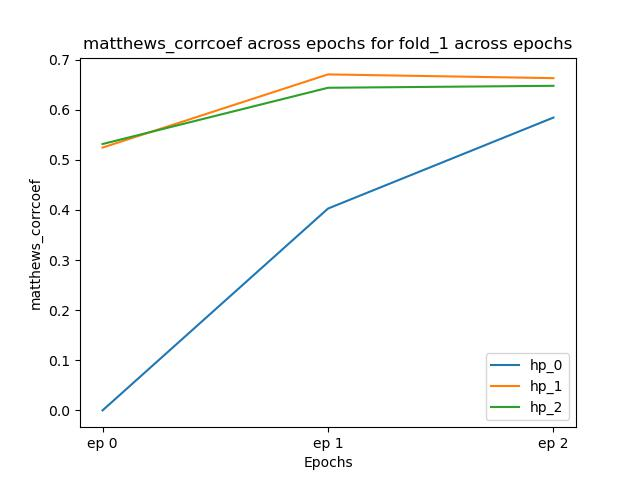
\includegraphics[scale = 0.75]{fold_1/matthews_corrcoef}
\end{figure}
\subsection{recall\_score}
\begin{tabular}{lrrr}
\toprule
{} &   ep 0 &   ep 1 &   ep 2 \\
\midrule
hp\_0 &  0.000 &  0.952 &  0.855 \\
hp\_1 &  0.710 &  0.871 &  0.774 \\
hp\_2 &  0.581 &  0.774 &  0.758 \\
\bottomrule
\end{tabular}

\begin{figure}[H]
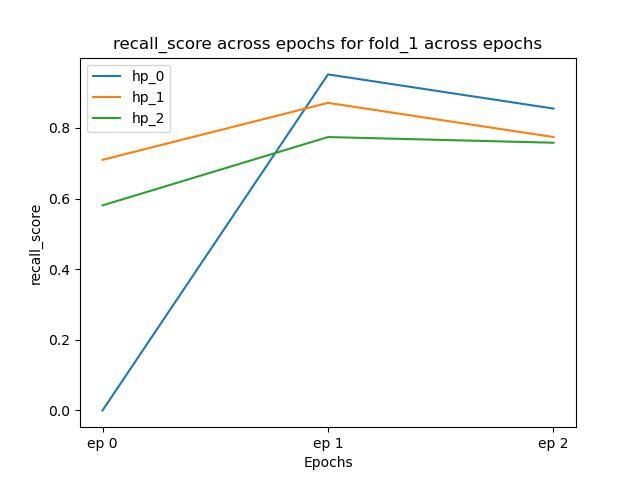
\includegraphics[scale = 0.75]{fold_1/recall_score}
\end{figure}
\section{fold\_2}
\subsection{train\_loss}
\begin{tabular}{lrrr}
\toprule
{} &   ep 0 &   ep 1 &   ep 2 \\
\midrule
hp\_0 &  0.740 &  0.621 &  0.685 \\
hp\_1 &  0.698 &  0.302 &  0.017 \\
hp\_2 &  0.697 &  0.449 &  0.094 \\
\bottomrule
\end{tabular}

\begin{figure}[H]
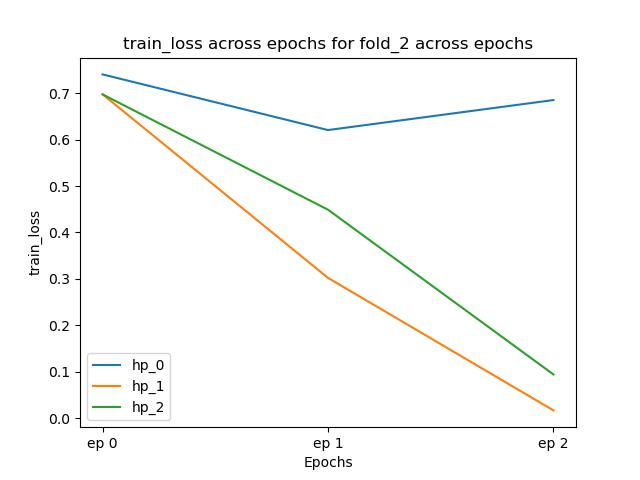
\includegraphics[scale = 0.75]{fold_2/train_loss}
\end{figure}
\subsection{test\_loss}
\begin{tabular}{lrrr}
\toprule
{} &   ep 0 &   ep 1 &   ep 2 \\
\midrule
hp\_0 &  0.664 &  0.543 &  0.686 \\
hp\_1 &  0.581 &  0.269 &  0.264 \\
hp\_2 &  0.599 &  0.350 &  0.245 \\
\bottomrule
\end{tabular}

\begin{figure}[H]
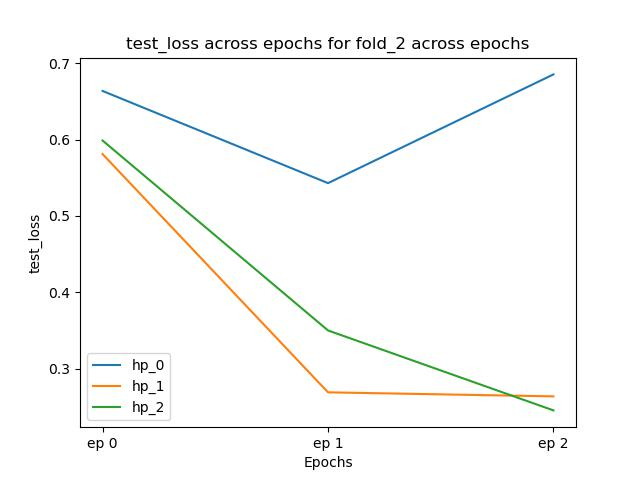
\includegraphics[scale = 0.75]{fold_2/test_loss}
\end{figure}
\subsection{accuracy\_score}
\begin{tabular}{lrrr}
\toprule
{} &   ep 0 &   ep 1 &   ep 2 \\
\midrule
hp\_0 &  0.595 &  0.750 &  0.586 \\
hp\_1 &  0.819 &  0.905 &  0.879 \\
hp\_2 &  0.776 &  0.897 &  0.879 \\
\bottomrule
\end{tabular}

\begin{figure}[H]
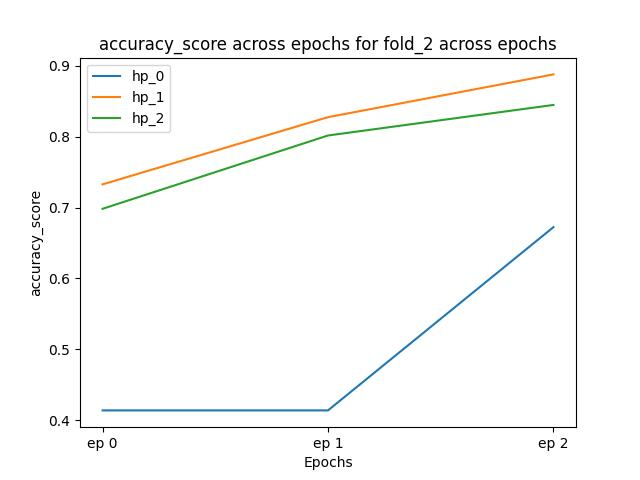
\includegraphics[scale = 0.75]{fold_2/accuracy_score}
\end{figure}
\subsection{f1\_score}
\begin{tabular}{lrrr}
\toprule
{} &   ep 0 &   ep 1 &   ep 2 \\
\midrule
hp\_0 &  0.041 &  0.707 &  0.000 \\
hp\_1 &  0.753 &  0.874 &  0.865 \\
hp\_2 &  0.705 &  0.860 &  0.848 \\
\bottomrule
\end{tabular}

\begin{figure}[H]
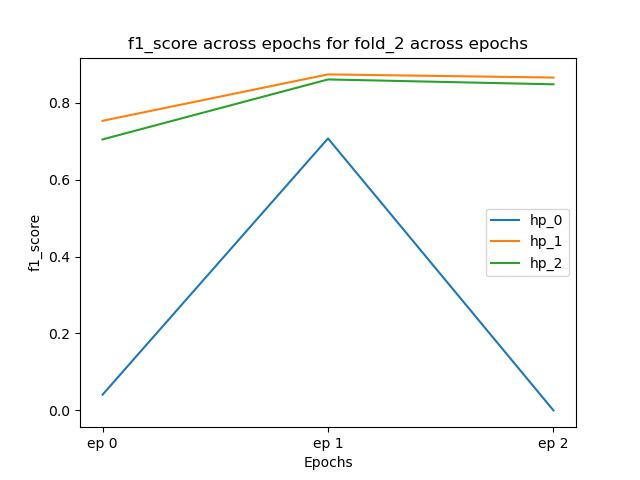
\includegraphics[scale = 0.75]{fold_2/f1_score}
\end{figure}
\subsection{precision\_score}
\begin{tabular}{lrrr}
\toprule
{} &   ep 0 &   ep 1 &   ep 2 \\
\midrule
hp\_0 &  1.000 &  0.686 &  0.000 \\
hp\_1 &  0.865 &  0.974 &  0.804 \\
hp\_2 &  0.775 &  0.974 &  0.886 \\
\bottomrule
\end{tabular}

\begin{figure}[H]
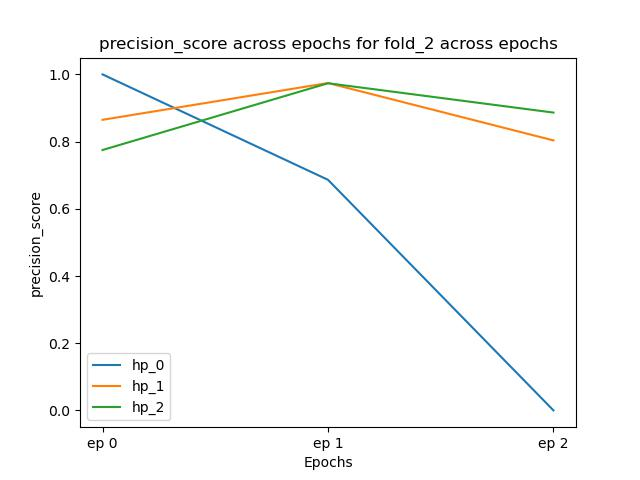
\includegraphics[scale = 0.75]{fold_2/precision_score}
\end{figure}
\subsection{matthews\_corrcoef}
\begin{tabular}{lrrr}
\toprule
{} &   ep 0 &   ep 1 &   ep 2 \\
\midrule
hp\_0 &  0.111 &  0.490 &  0.000 \\
hp\_1 &  0.627 &  0.810 &  0.765 \\
hp\_2 &  0.532 &  0.793 &  0.750 \\
\bottomrule
\end{tabular}

\begin{figure}[H]
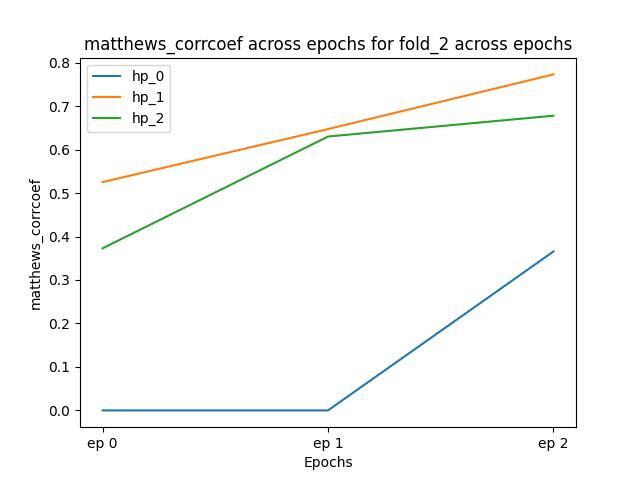
\includegraphics[scale = 0.75]{fold_2/matthews_corrcoef}
\end{figure}
\subsection{recall\_score}
\begin{tabular}{lrrr}
\toprule
{} &   ep 0 &   ep 1 &   ep 2 \\
\midrule
hp\_0 &  0.021 &  0.729 &  0.000 \\
hp\_1 &  0.667 &  0.792 &  0.938 \\
hp\_2 &  0.646 &  0.771 &  0.812 \\
\bottomrule
\end{tabular}

\begin{figure}[H]
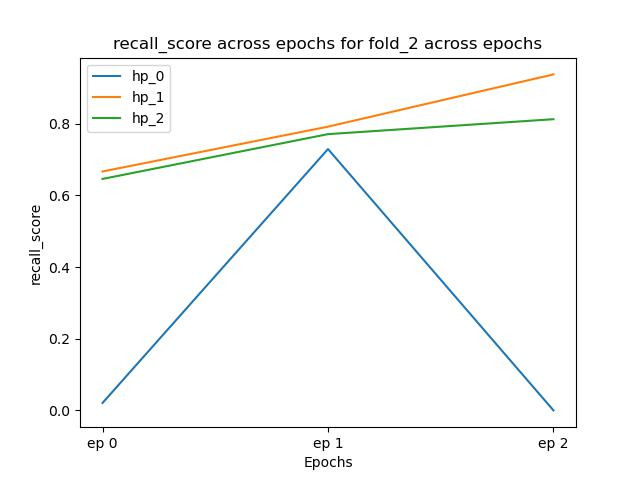
\includegraphics[scale = 0.75]{fold_2/recall_score}
\end{figure}
\end{document}
